\chapter{Rocketry}


Basic principles
	Can only throw what you carry (fuel needs fuel)
	Lots of fuel for small payload
	Third law
	[THIRD LAW GRAPHIC]


Rockets propel hot gases, which recreates an equal an opposite reaction which pushes it forwards, even in a vacuum. 

Imagine a rocket with a bowling ball attached. If the bowling ball is backwards from the rocket, the rocket will move forwards. 

This is also true for shooting gas. While each gas particle is much lighter than a bowling ball, it's shot out a very high speed. 

Rockets carry their own oxidizer to allow for a chemical reaction to produce fire in a vacuum. 



\section{Types of rocket motors}

There are two main types of chemical rockets. 

One type is a \newterm{Solid Fuel Rocket}, which ignites a solid fuel-oxidizer mix. Once the solid fuel is ignited it can't be stopped until all of the fuel is exhausted.

	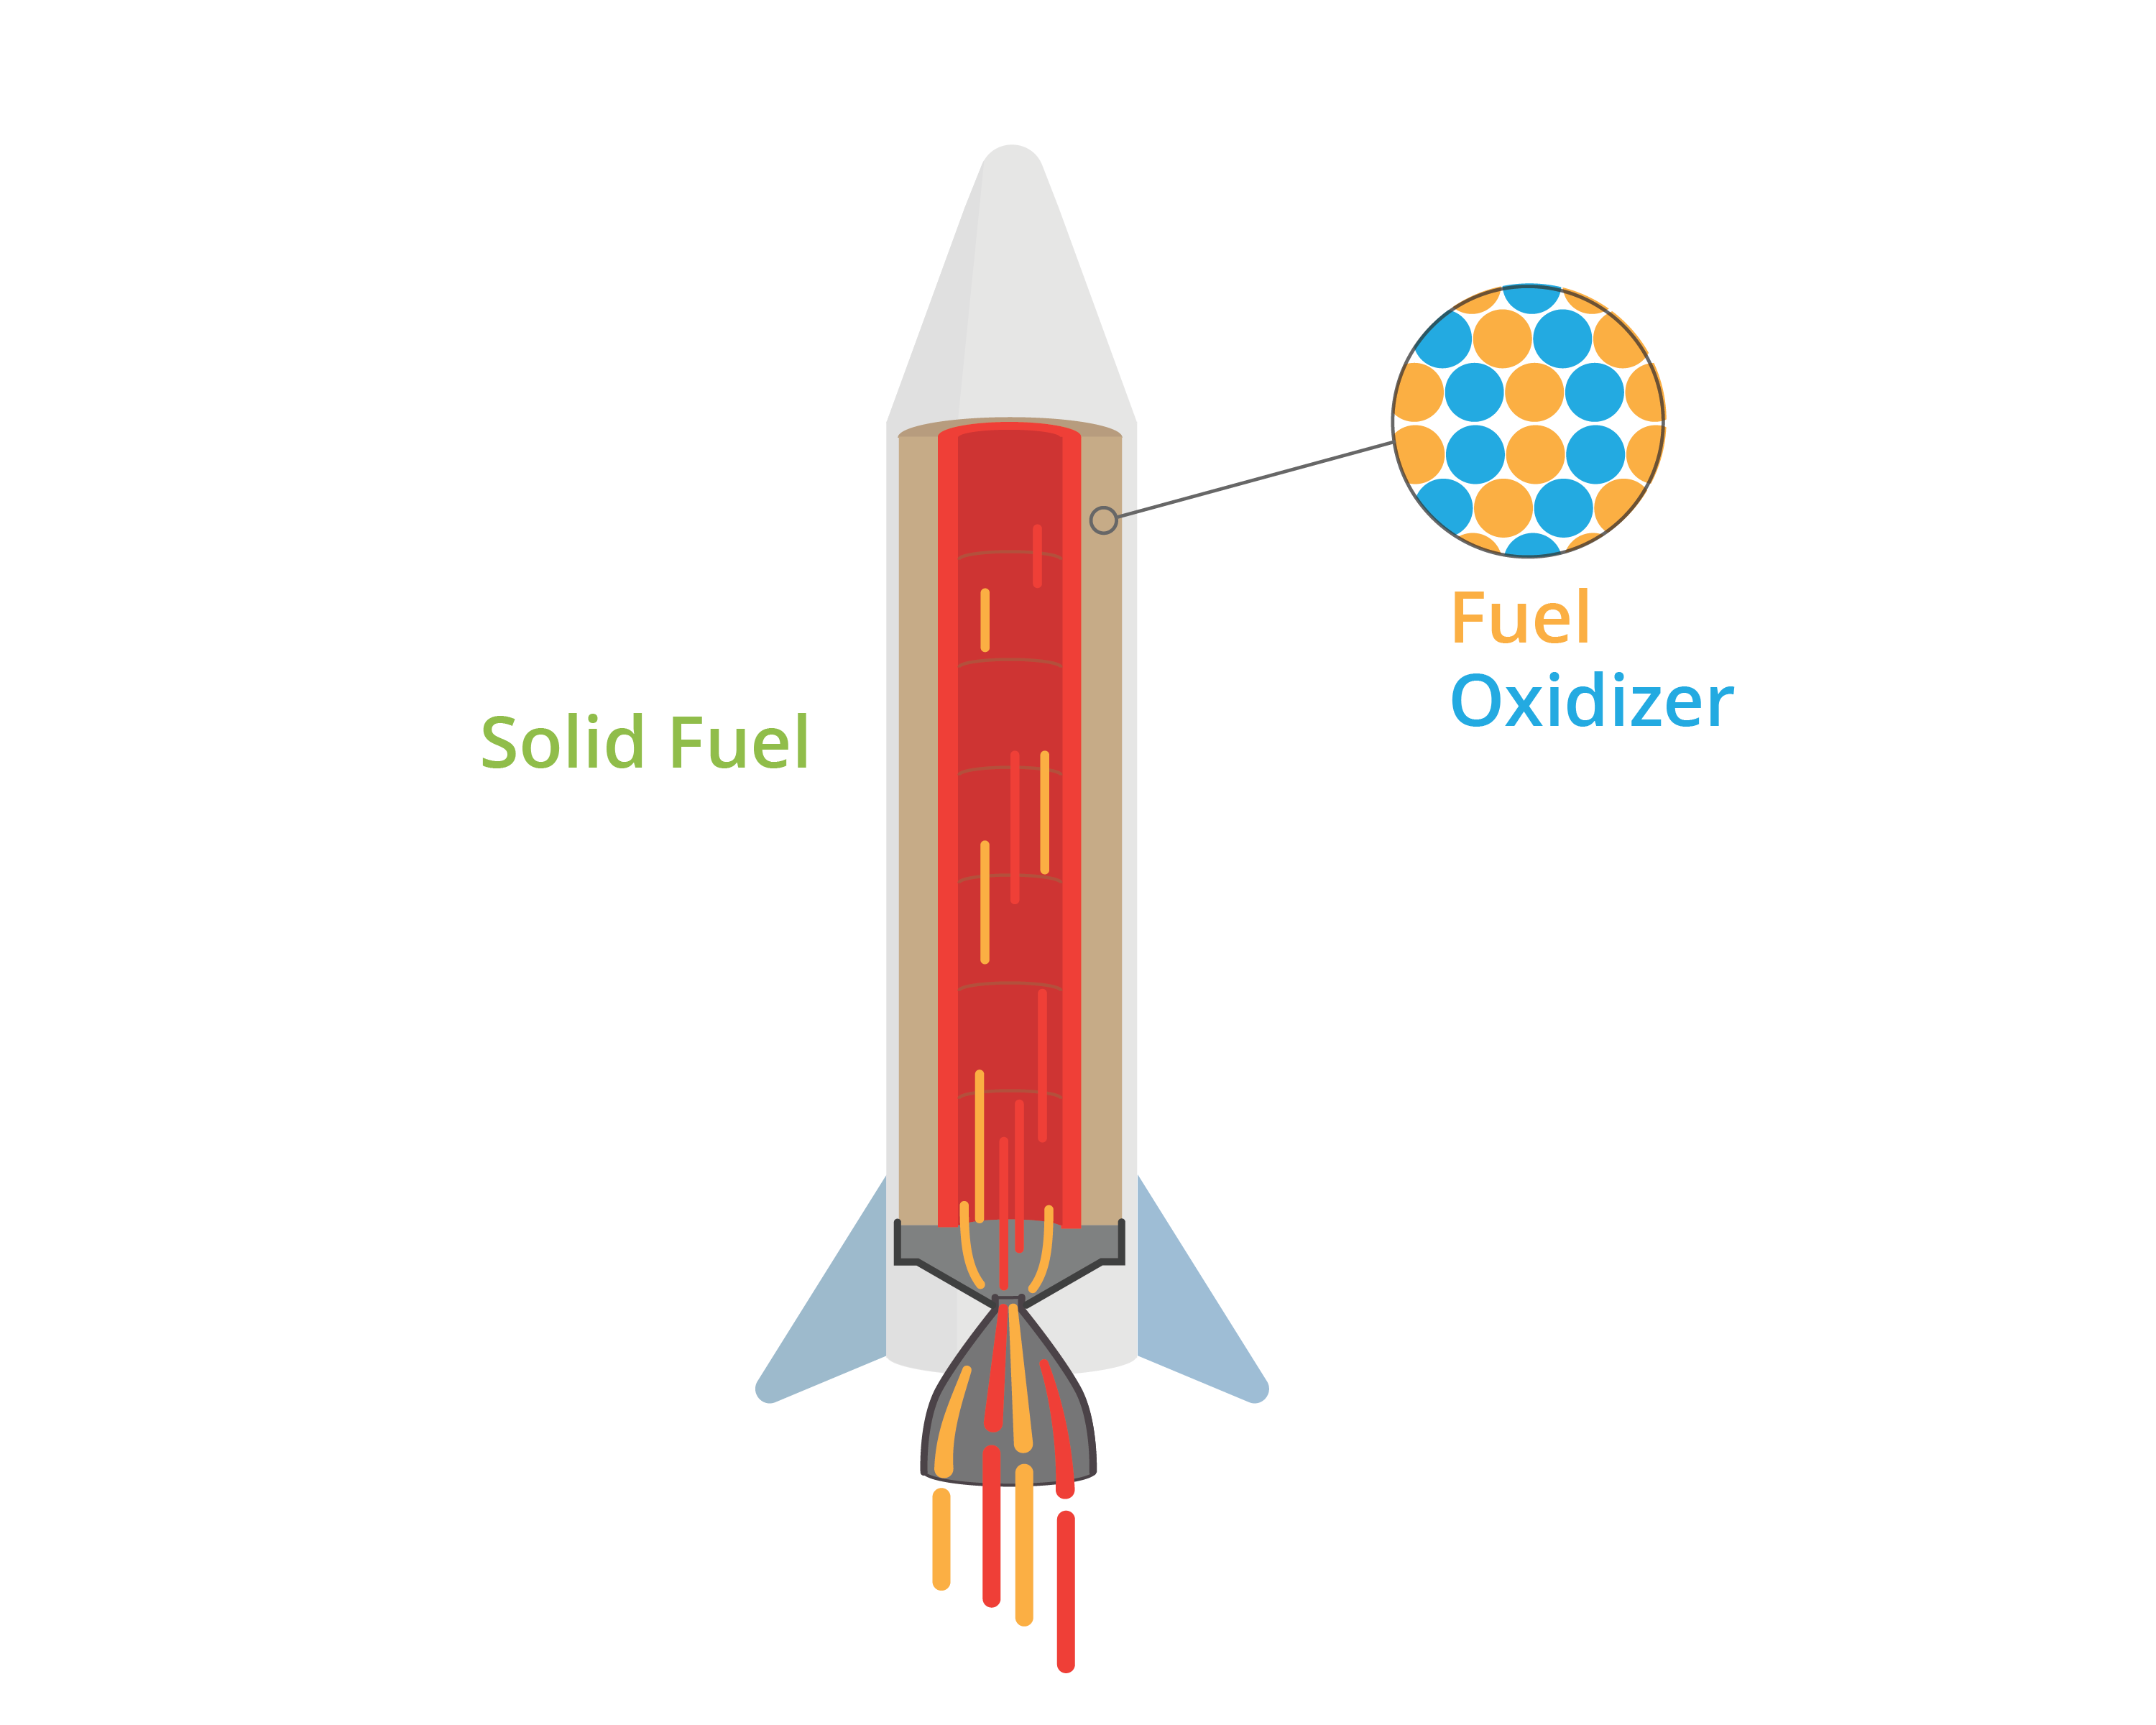
\includegraphics[width=0.75\textwidth]{solid.png}

The other main type of chemical rocket is called a \newterm{Liquid Fuel Rocket}
	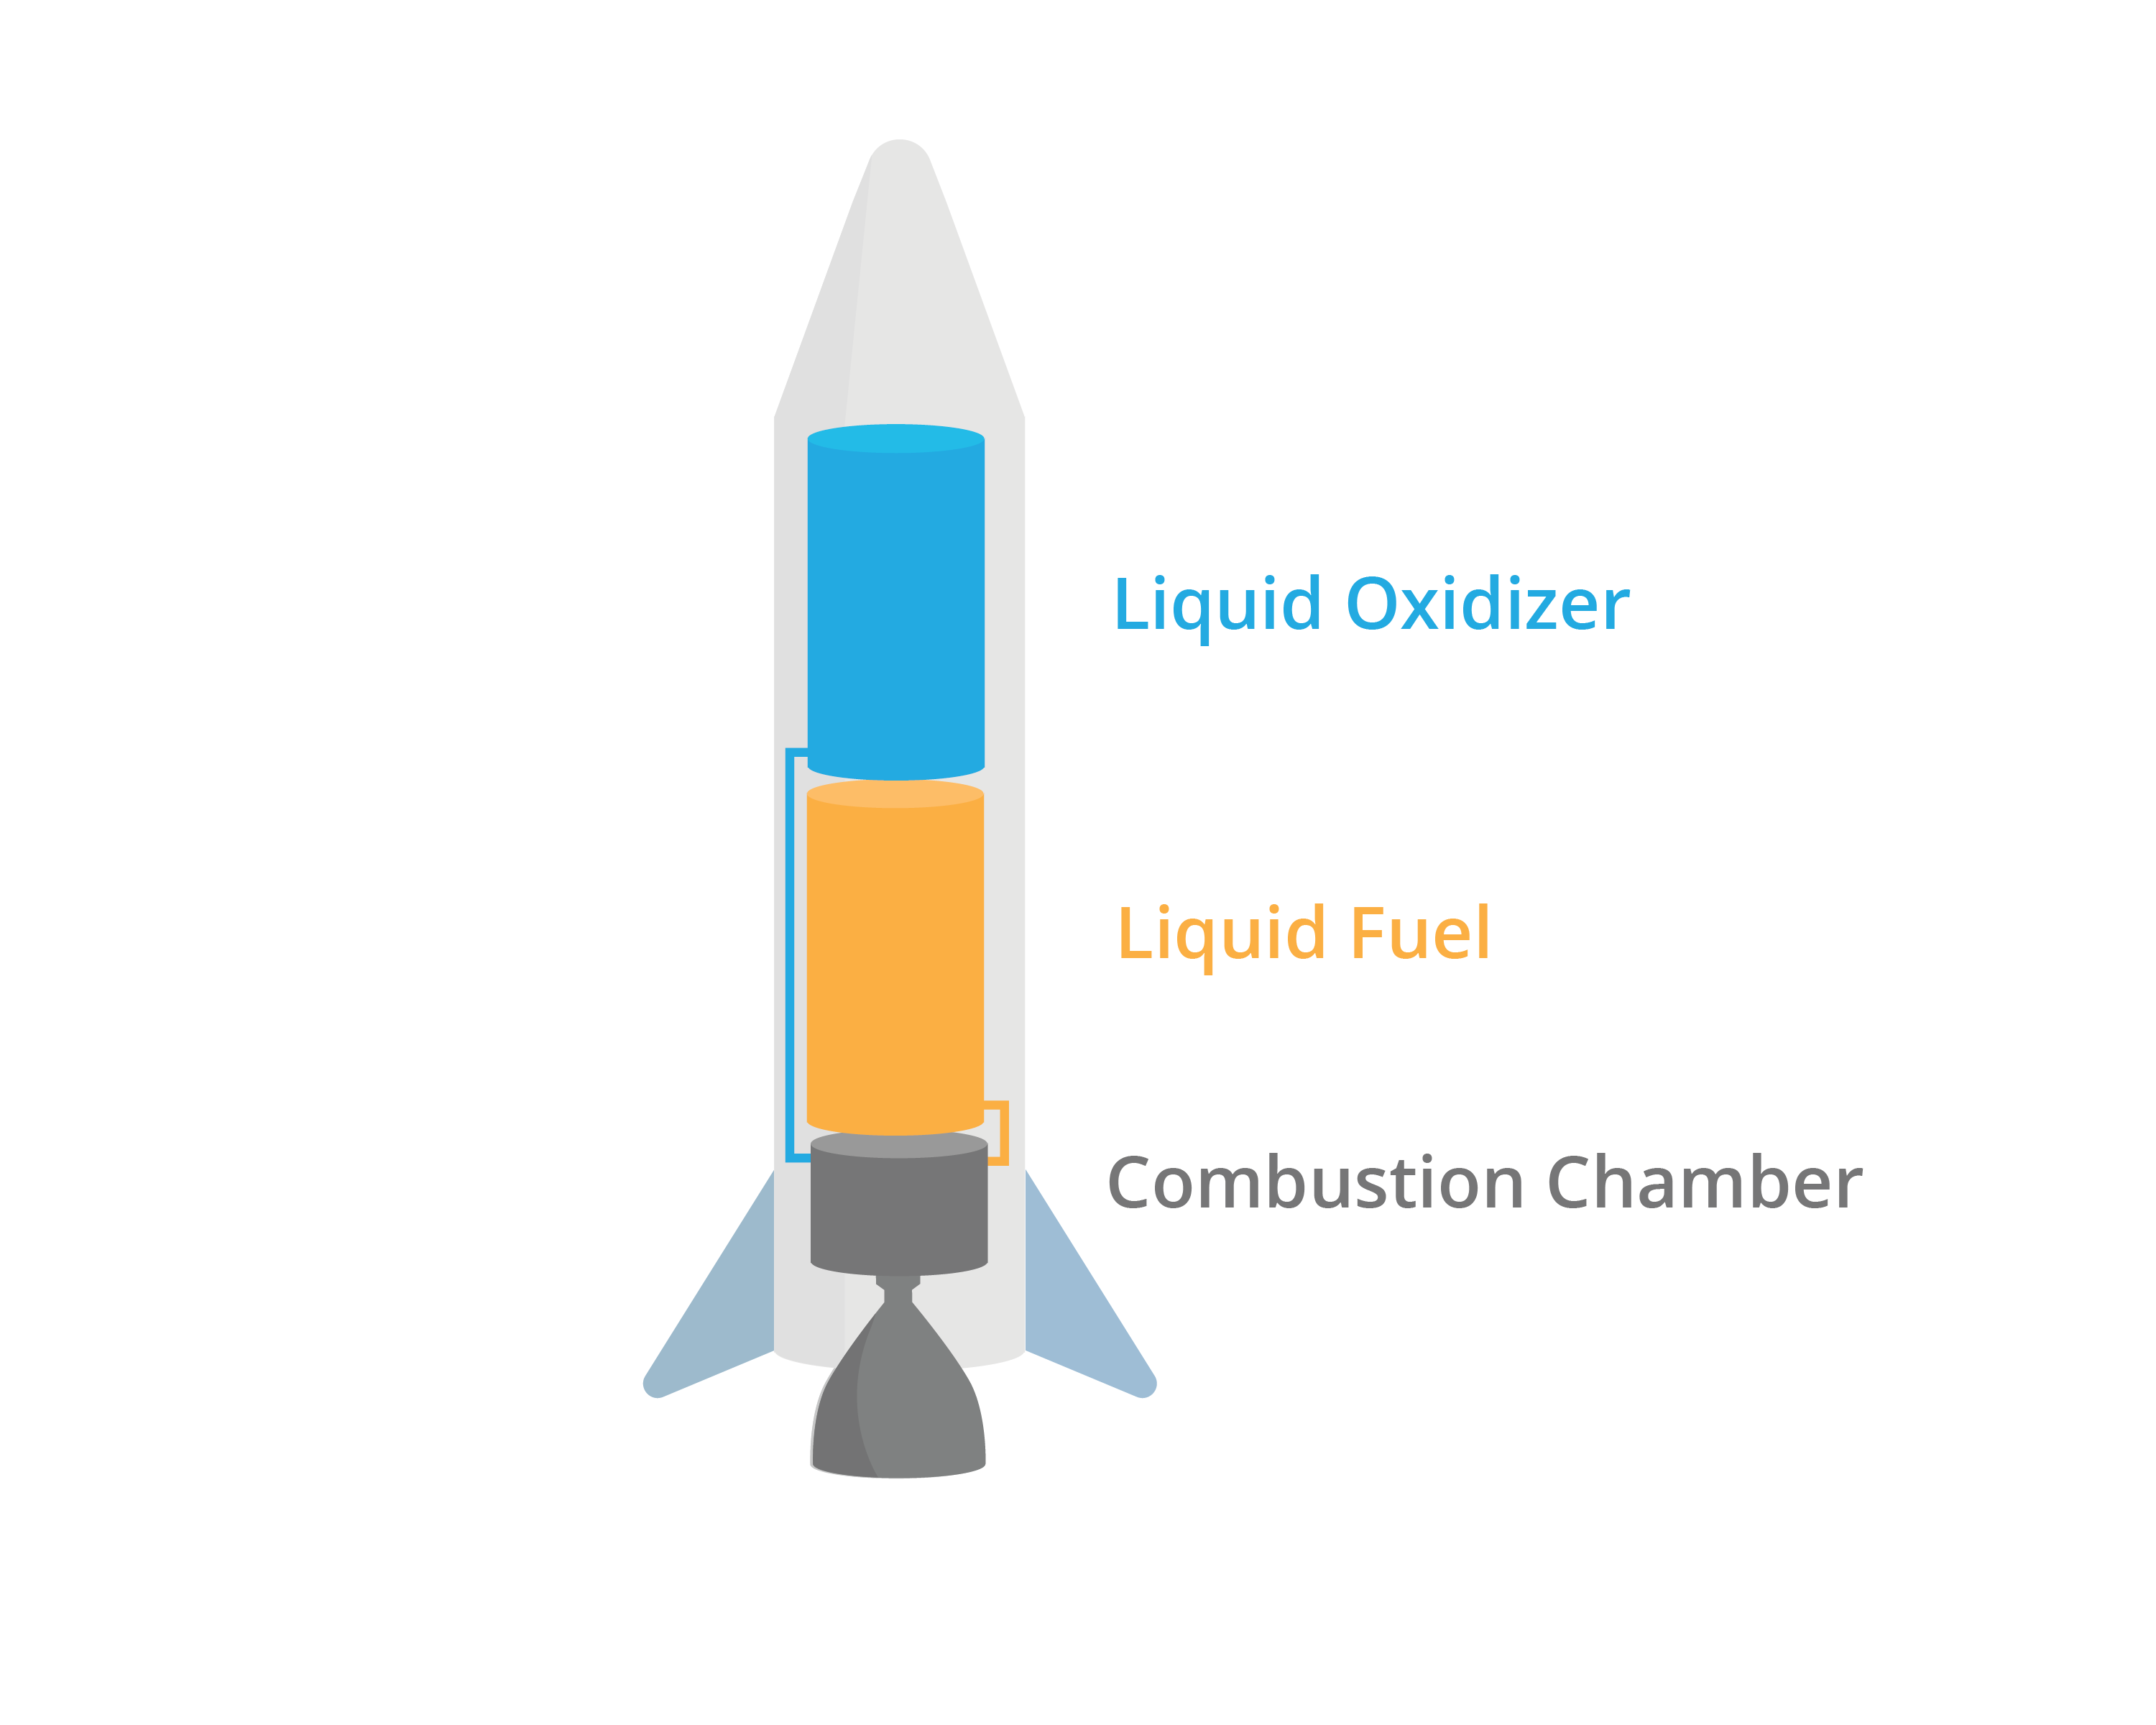
\includegraphics[width=0.75\textwidth]{liquid.png}

Liquid fuel rockets contain separate tanks for liquid fuel and oxidizer. Fuel pumps bring them both to a combustion chamber where they ignite and exit the rocket.


\section{Tyranny of the rocket equation}
	Chemical rockets can only burn the fuel that they bring with them. However, the more fuel you carry, the heavier the vehicle will be. 

		\newterm{staging}
		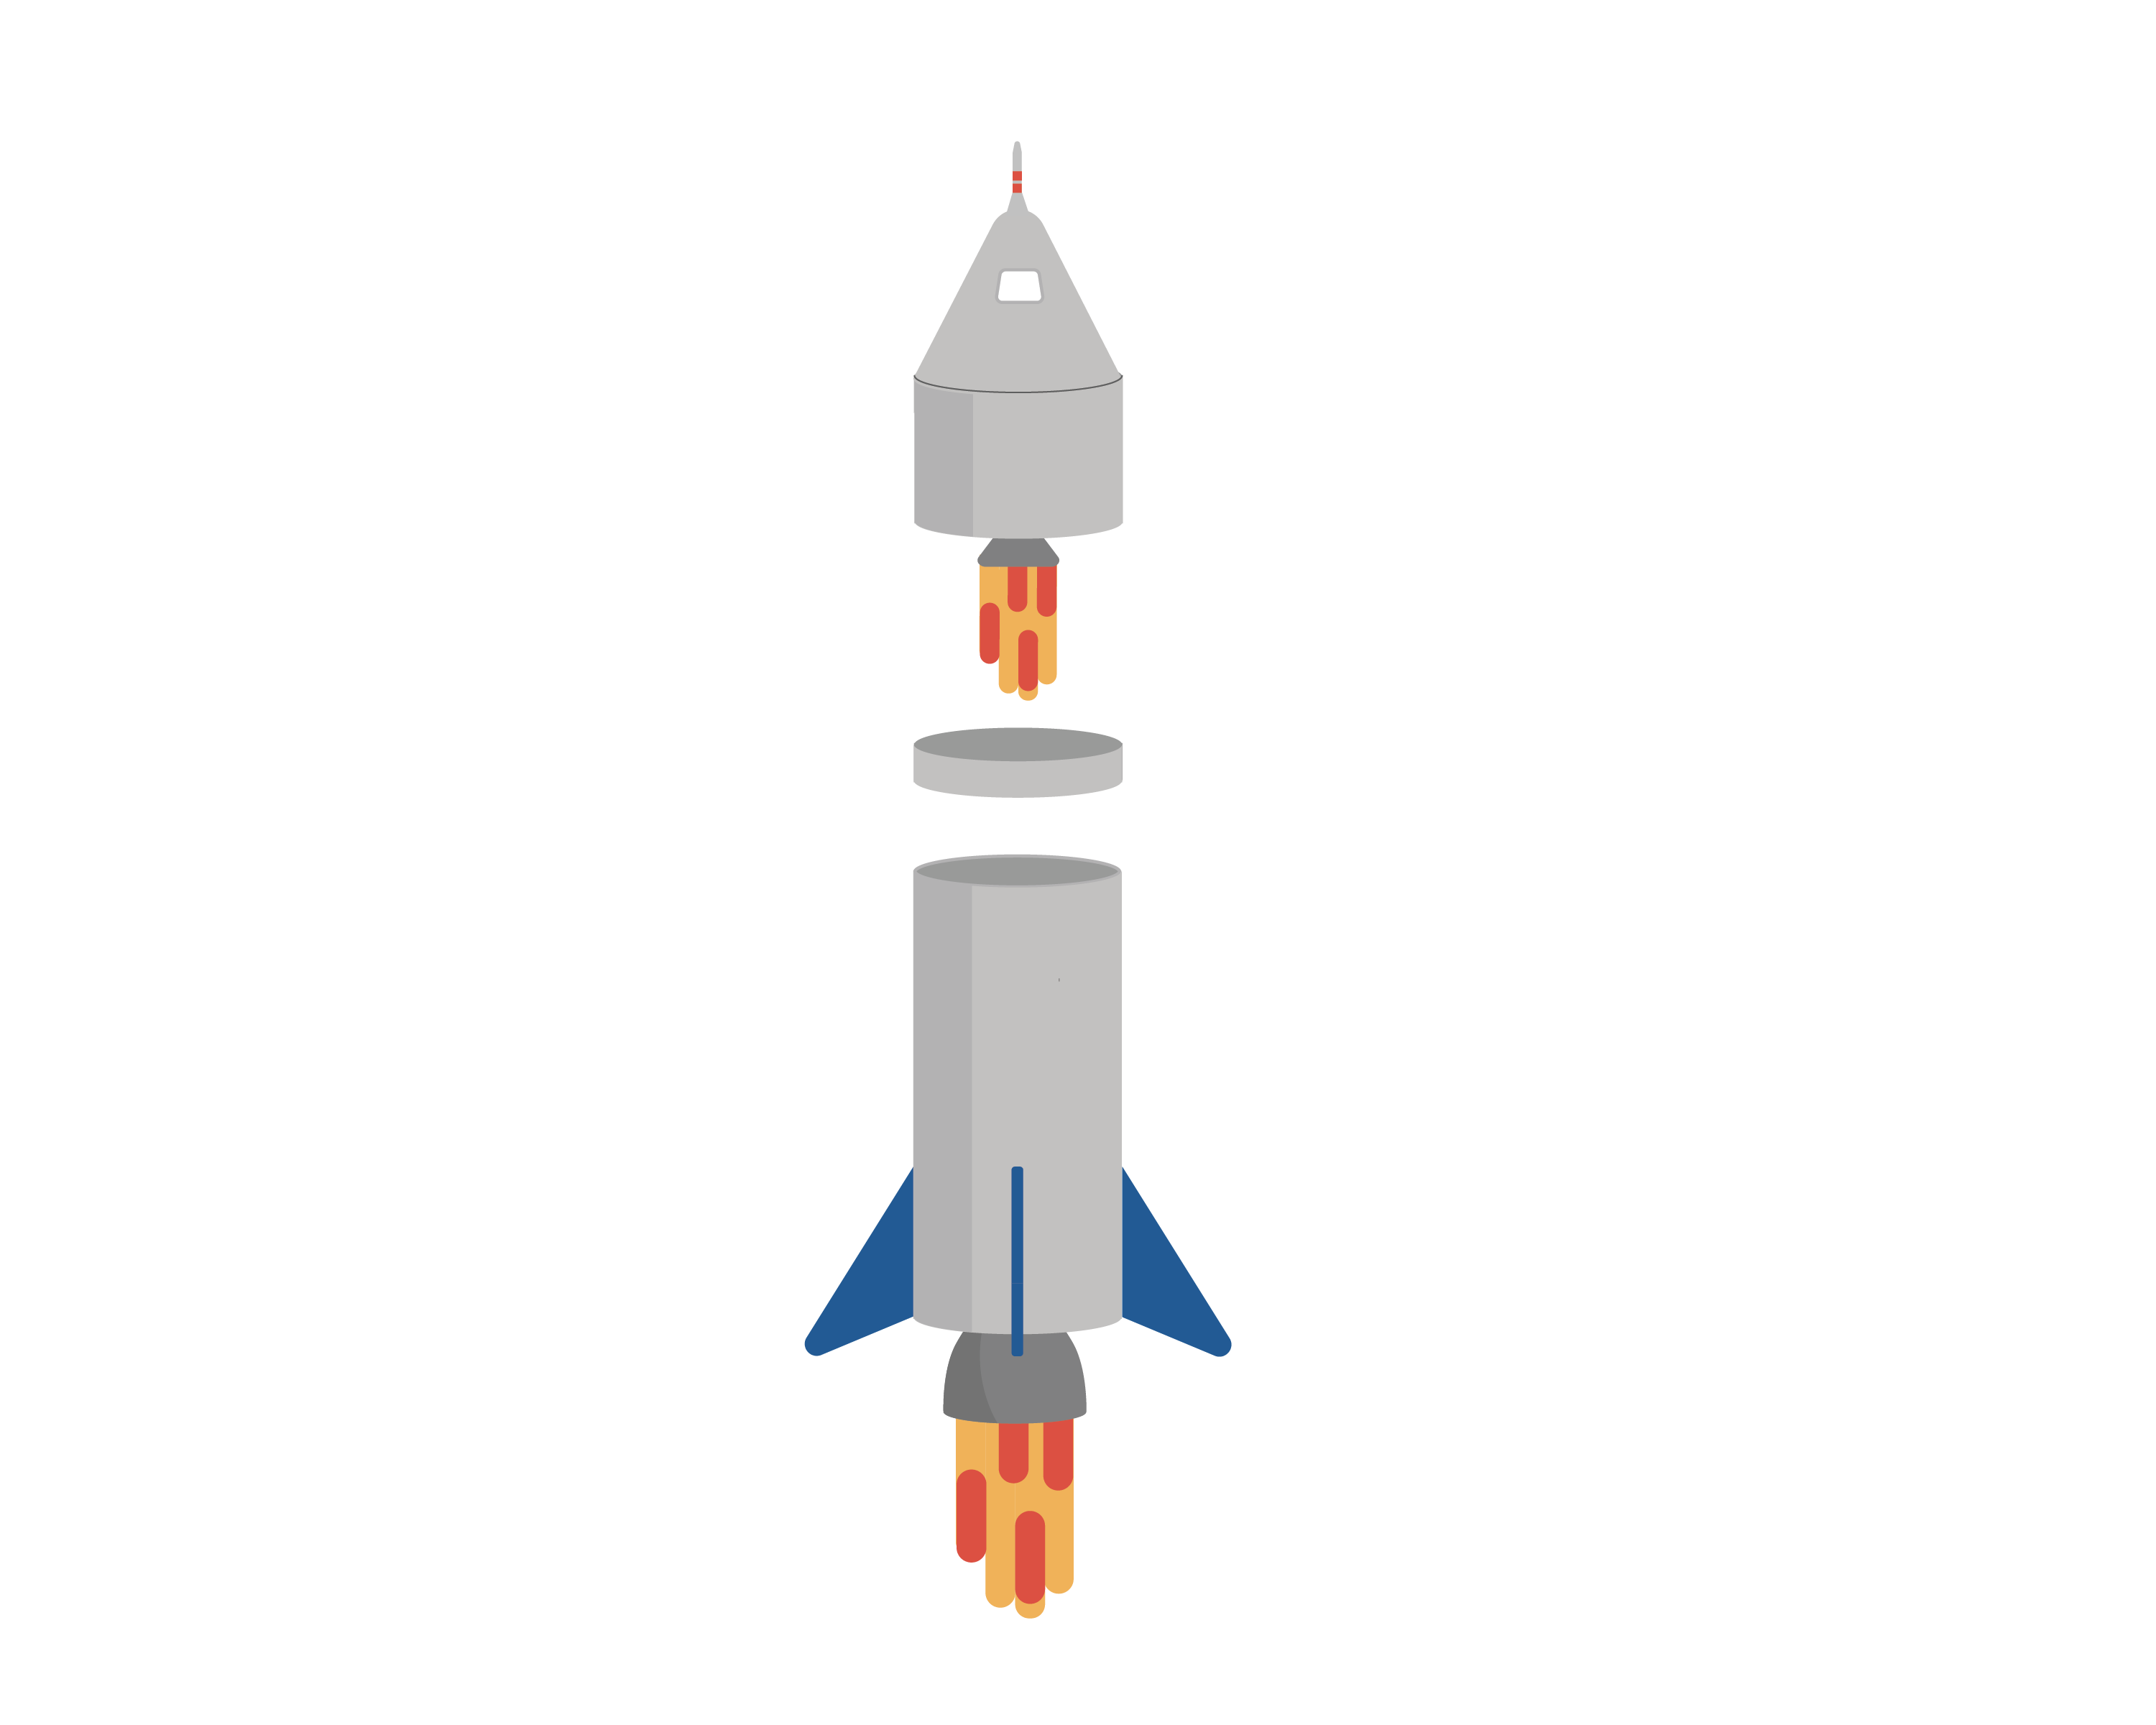
\includegraphics[width=0.75\textwidth]{staging.png}


		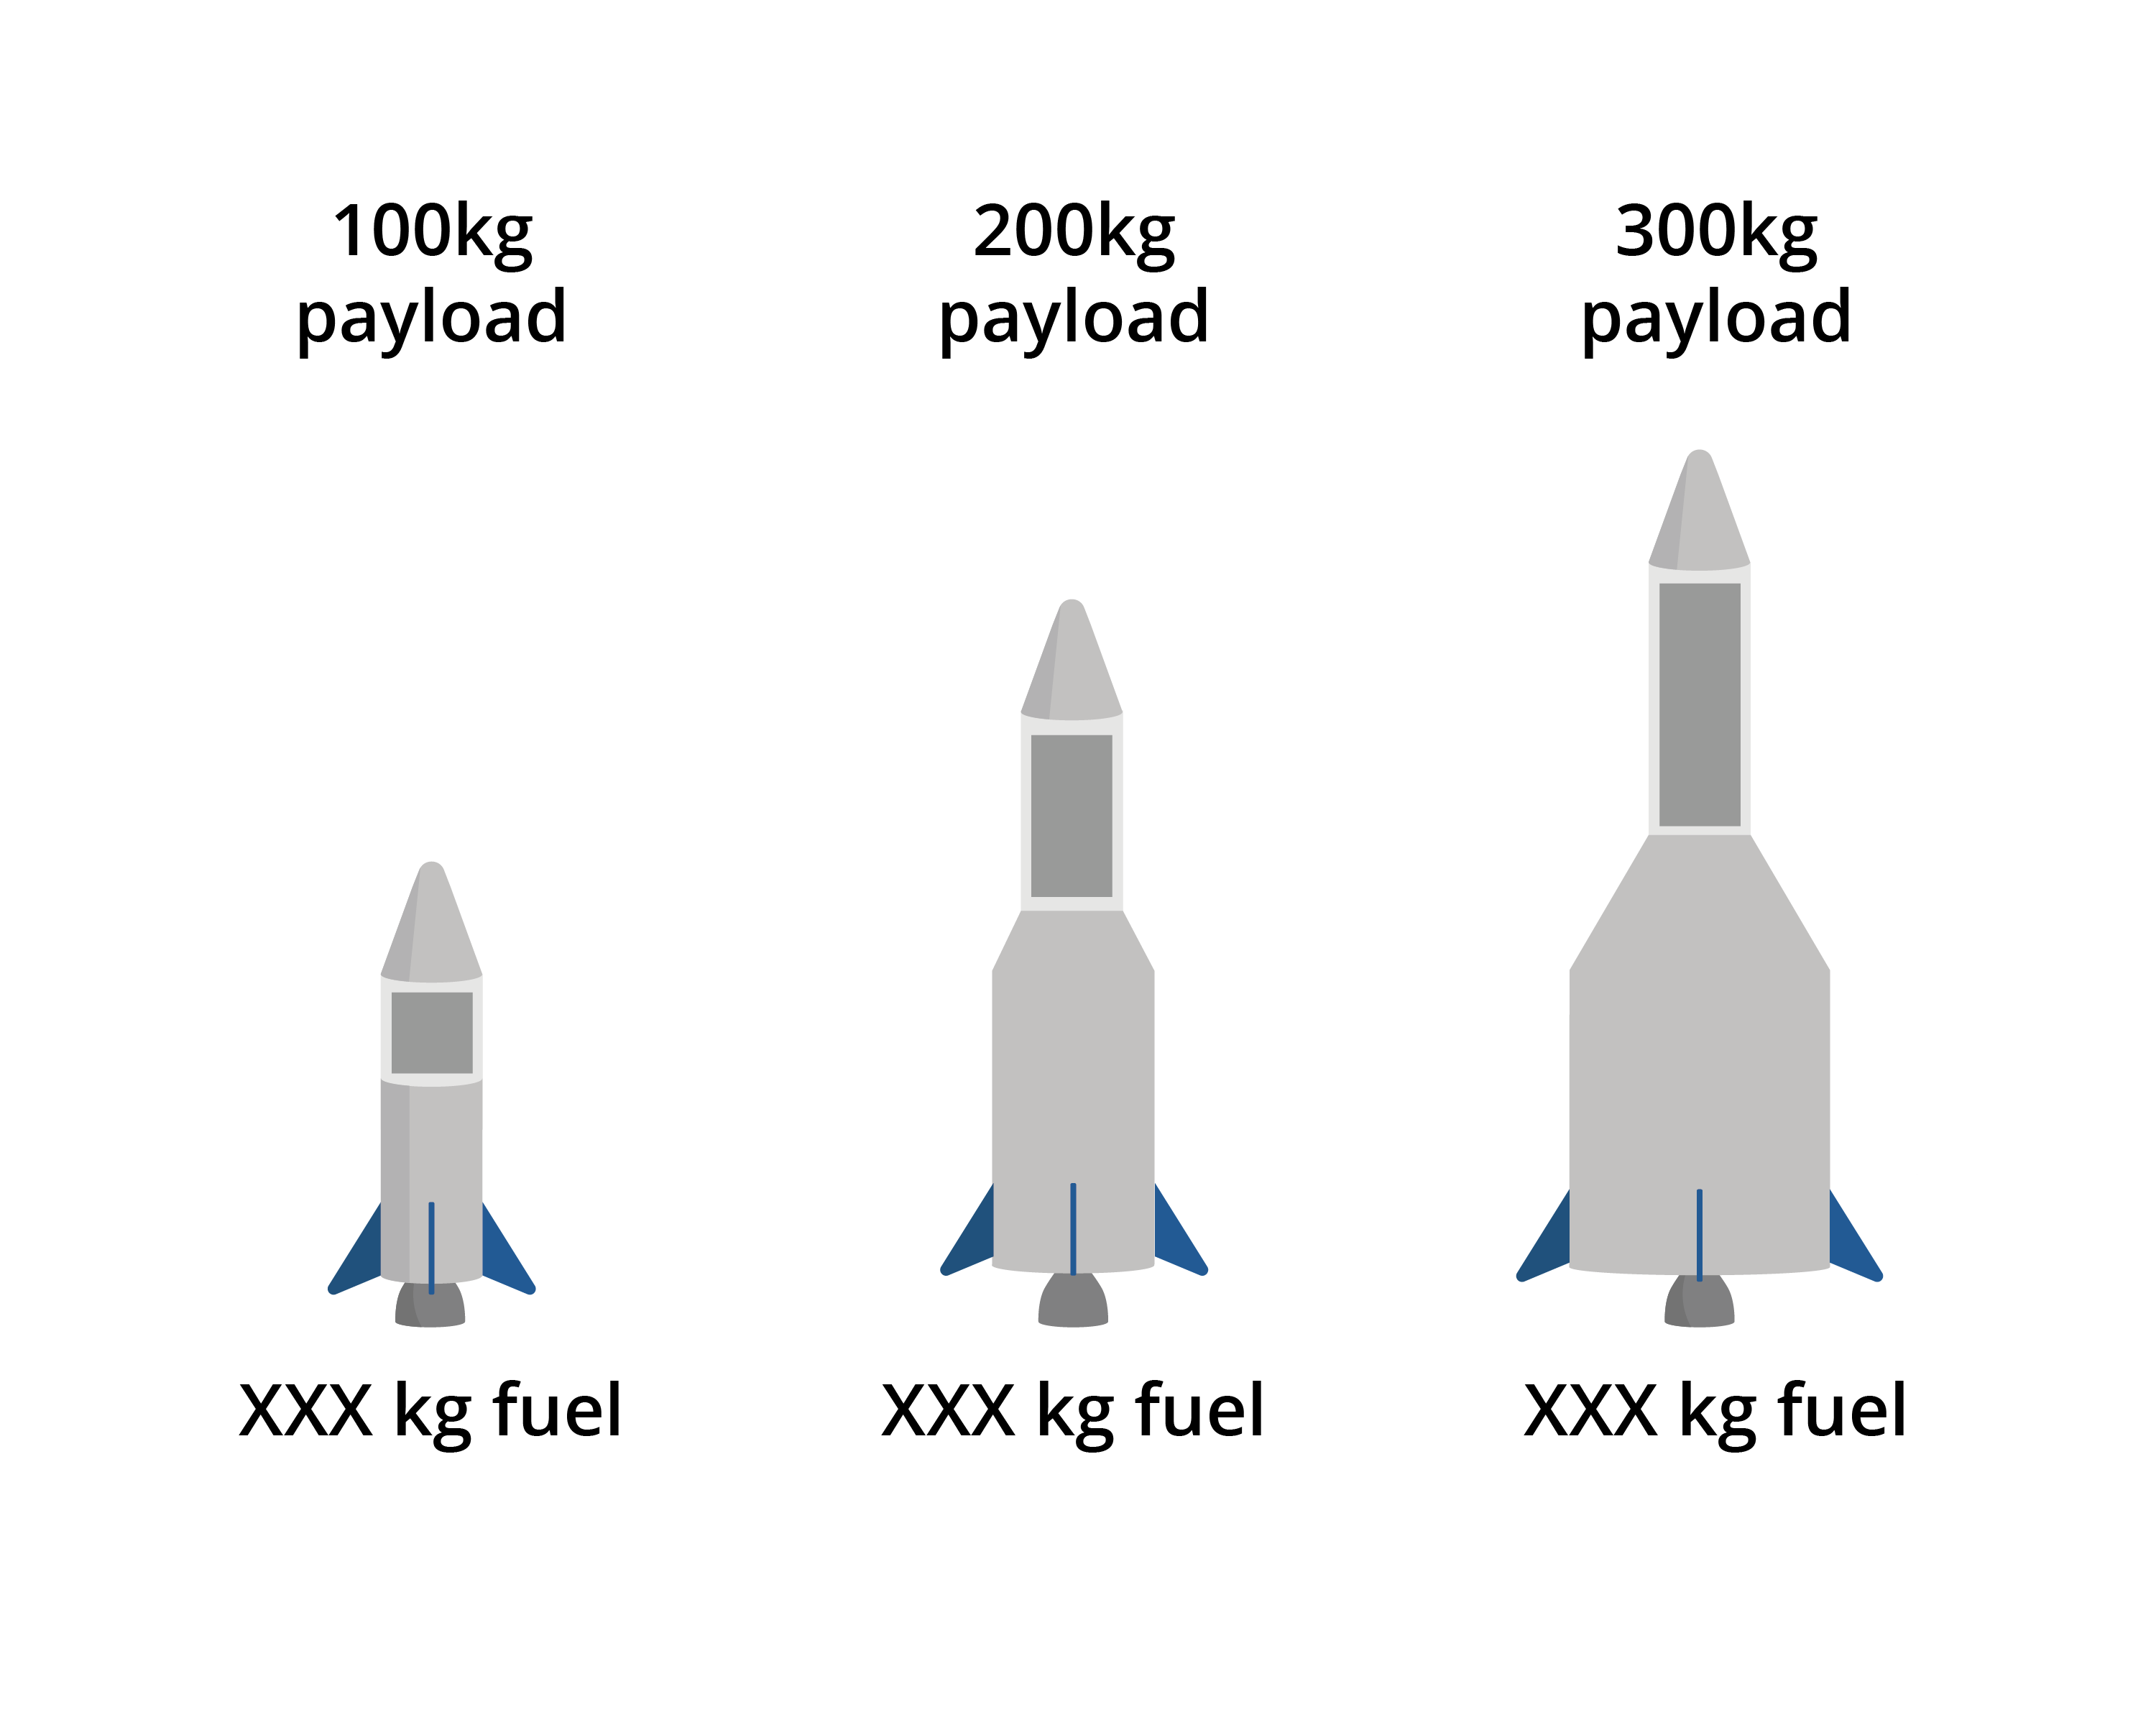
\includegraphics[width=0.75\textwidth]{rocketFuelWeight.png}


\section{Control in atmosphere}

There are several common ways that engineers have managed to control rockets' direction in the atmosphere. Usually, on-board sensors detect the orientation of the rocket, and can automatically adjust these controls to keep the rocket going the correct direction.

	
	One method is using \newterm{movable fins}.  [pros and cons]

	Another method of control uses a \newterm{gimbaled engine}. [pros and cons]
	
	A more outdated method is using \newterm{vernier engines}, which are two smaller engines that control attitude. However, this adds a lot of weight to the rocket, so they are less frequently used today. [pros and cons]

	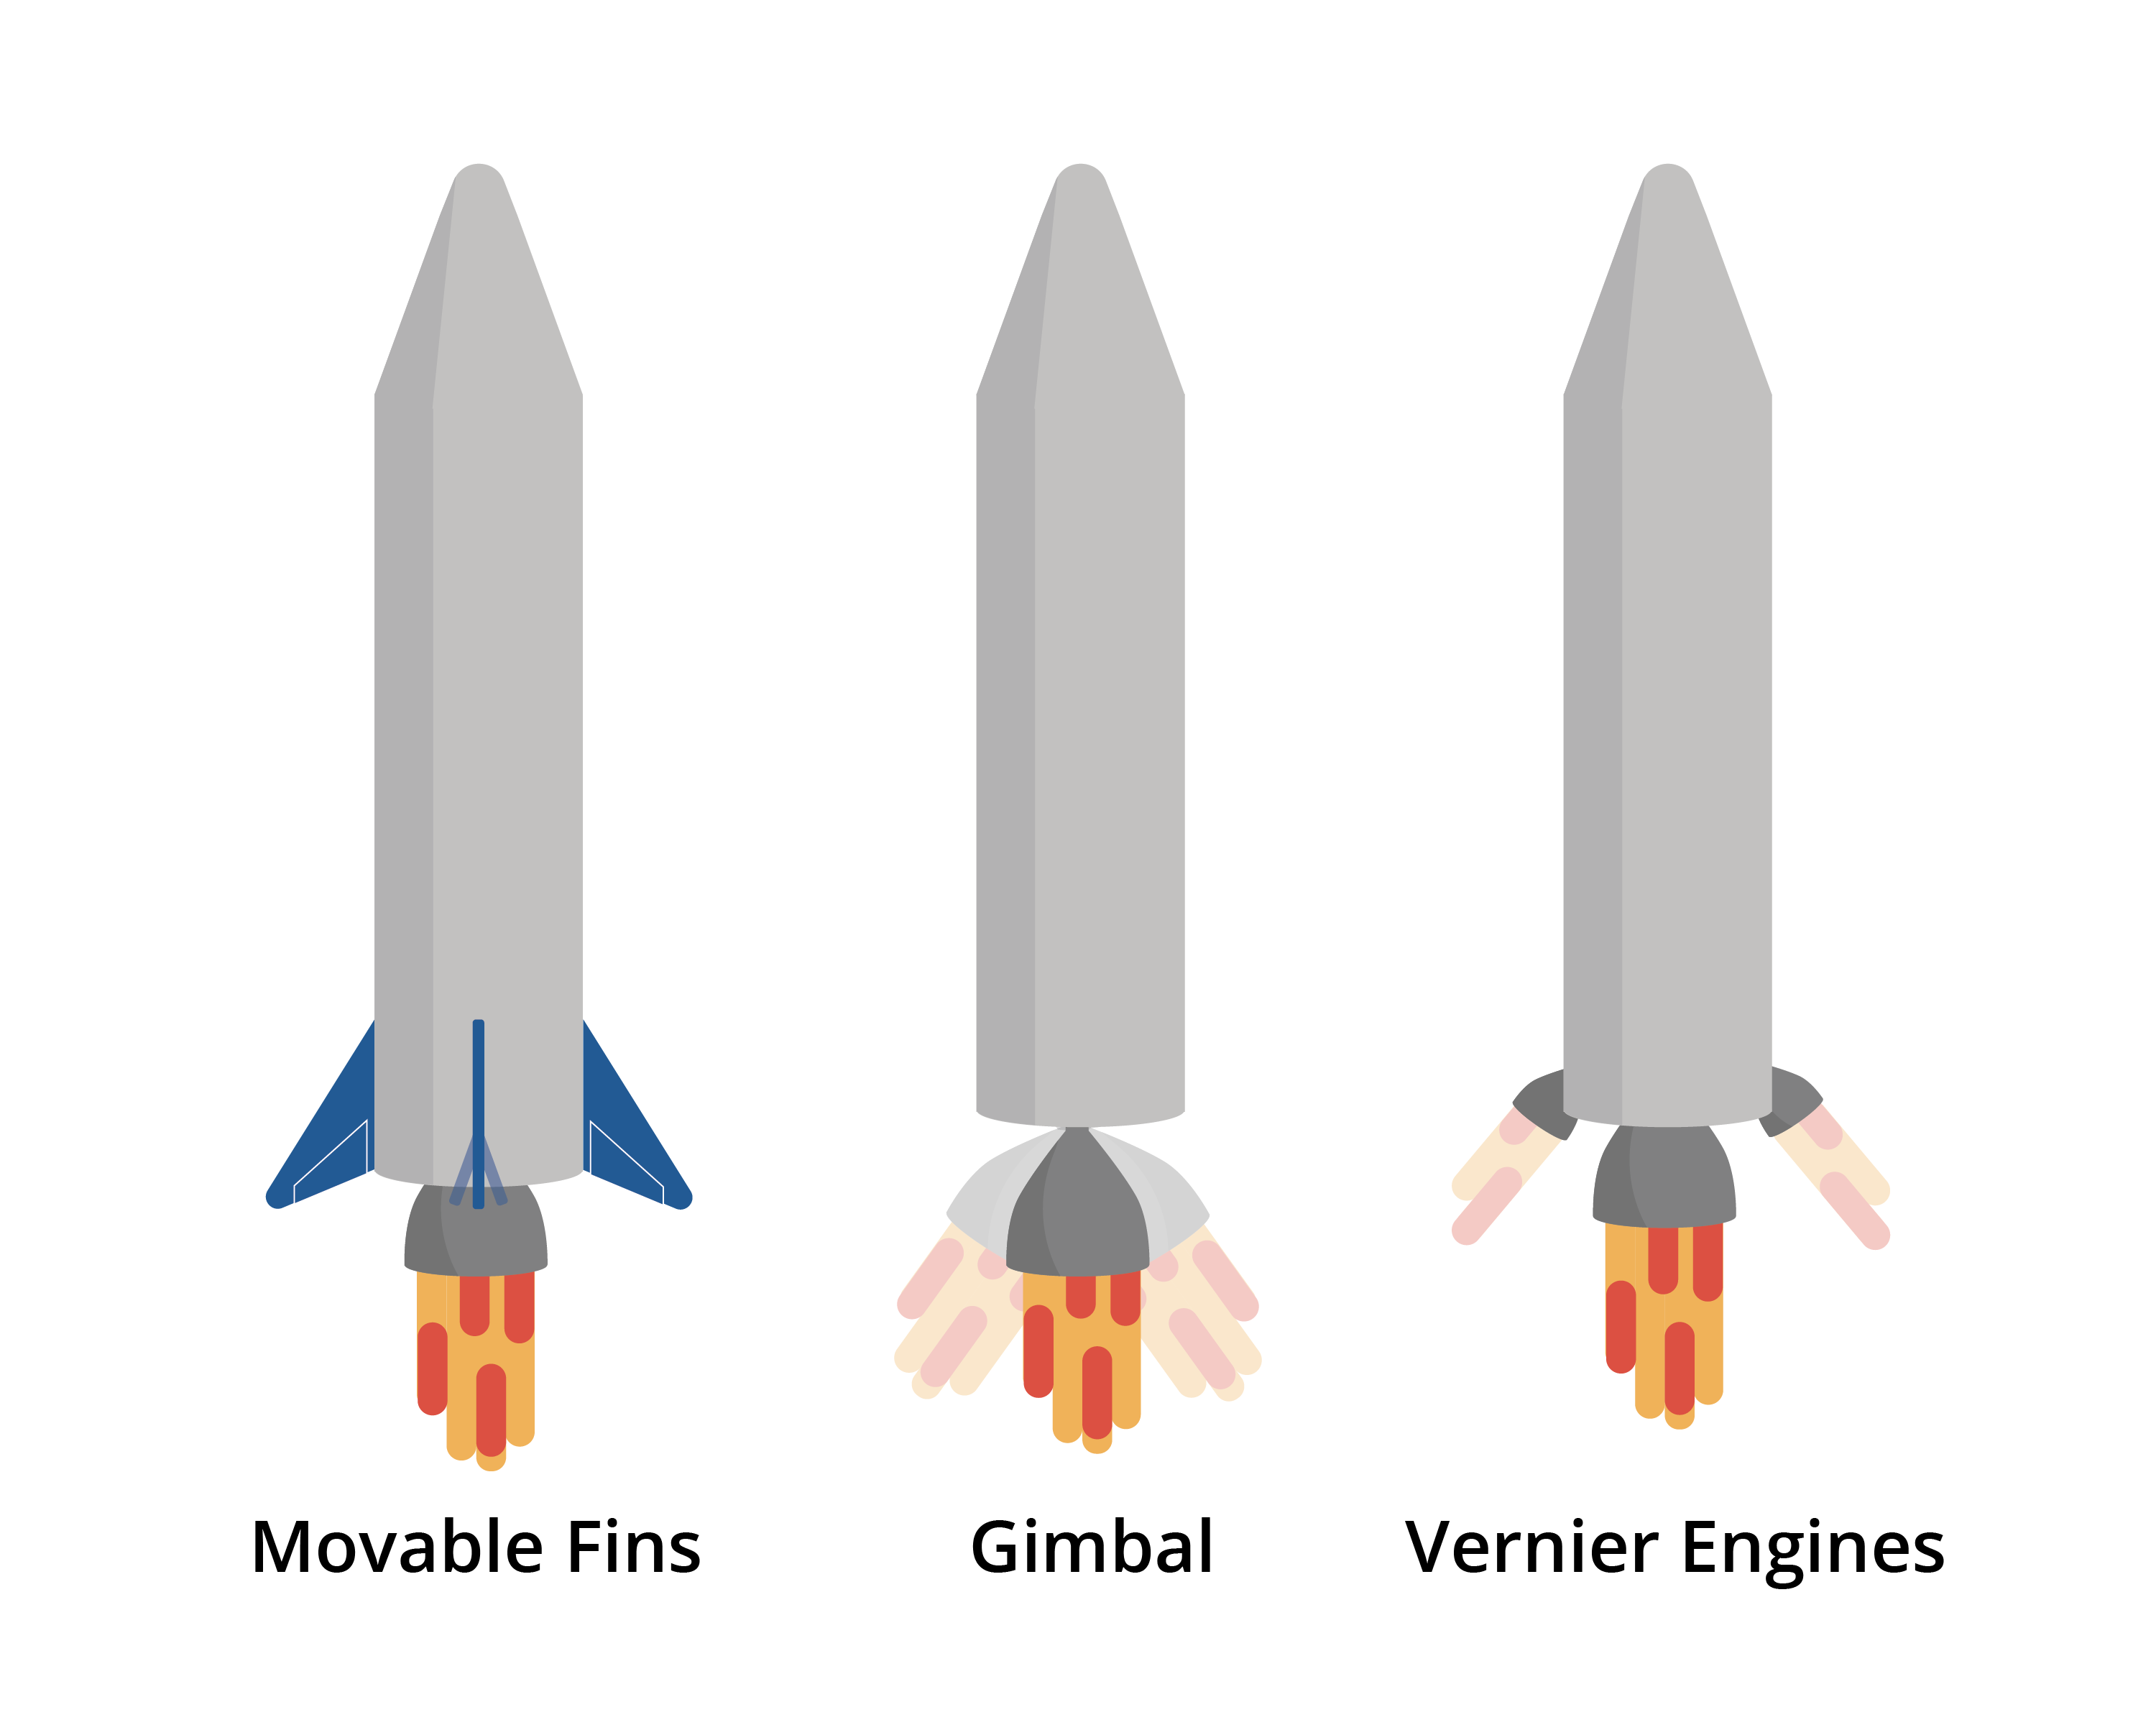
\includegraphics[width=0.75\textwidth]{control.png}


\section{Control in space}

The previous section describes ways that engineers control rockets in the atmosphere, but most rockets will end up in the vacuum of space. There are several common ways to adjust the orientation in space.

	One method is using \newterm{RCS thrusters}. 
	Another method called \newterm{reaction wheels} uses angular momentum to rotate the spacecraft. By accelerating and decelerating wheels on three axes, the spacecraft can rotate in any direction.

	A third common attitude control technology is \newterm{magnetASDFA}


	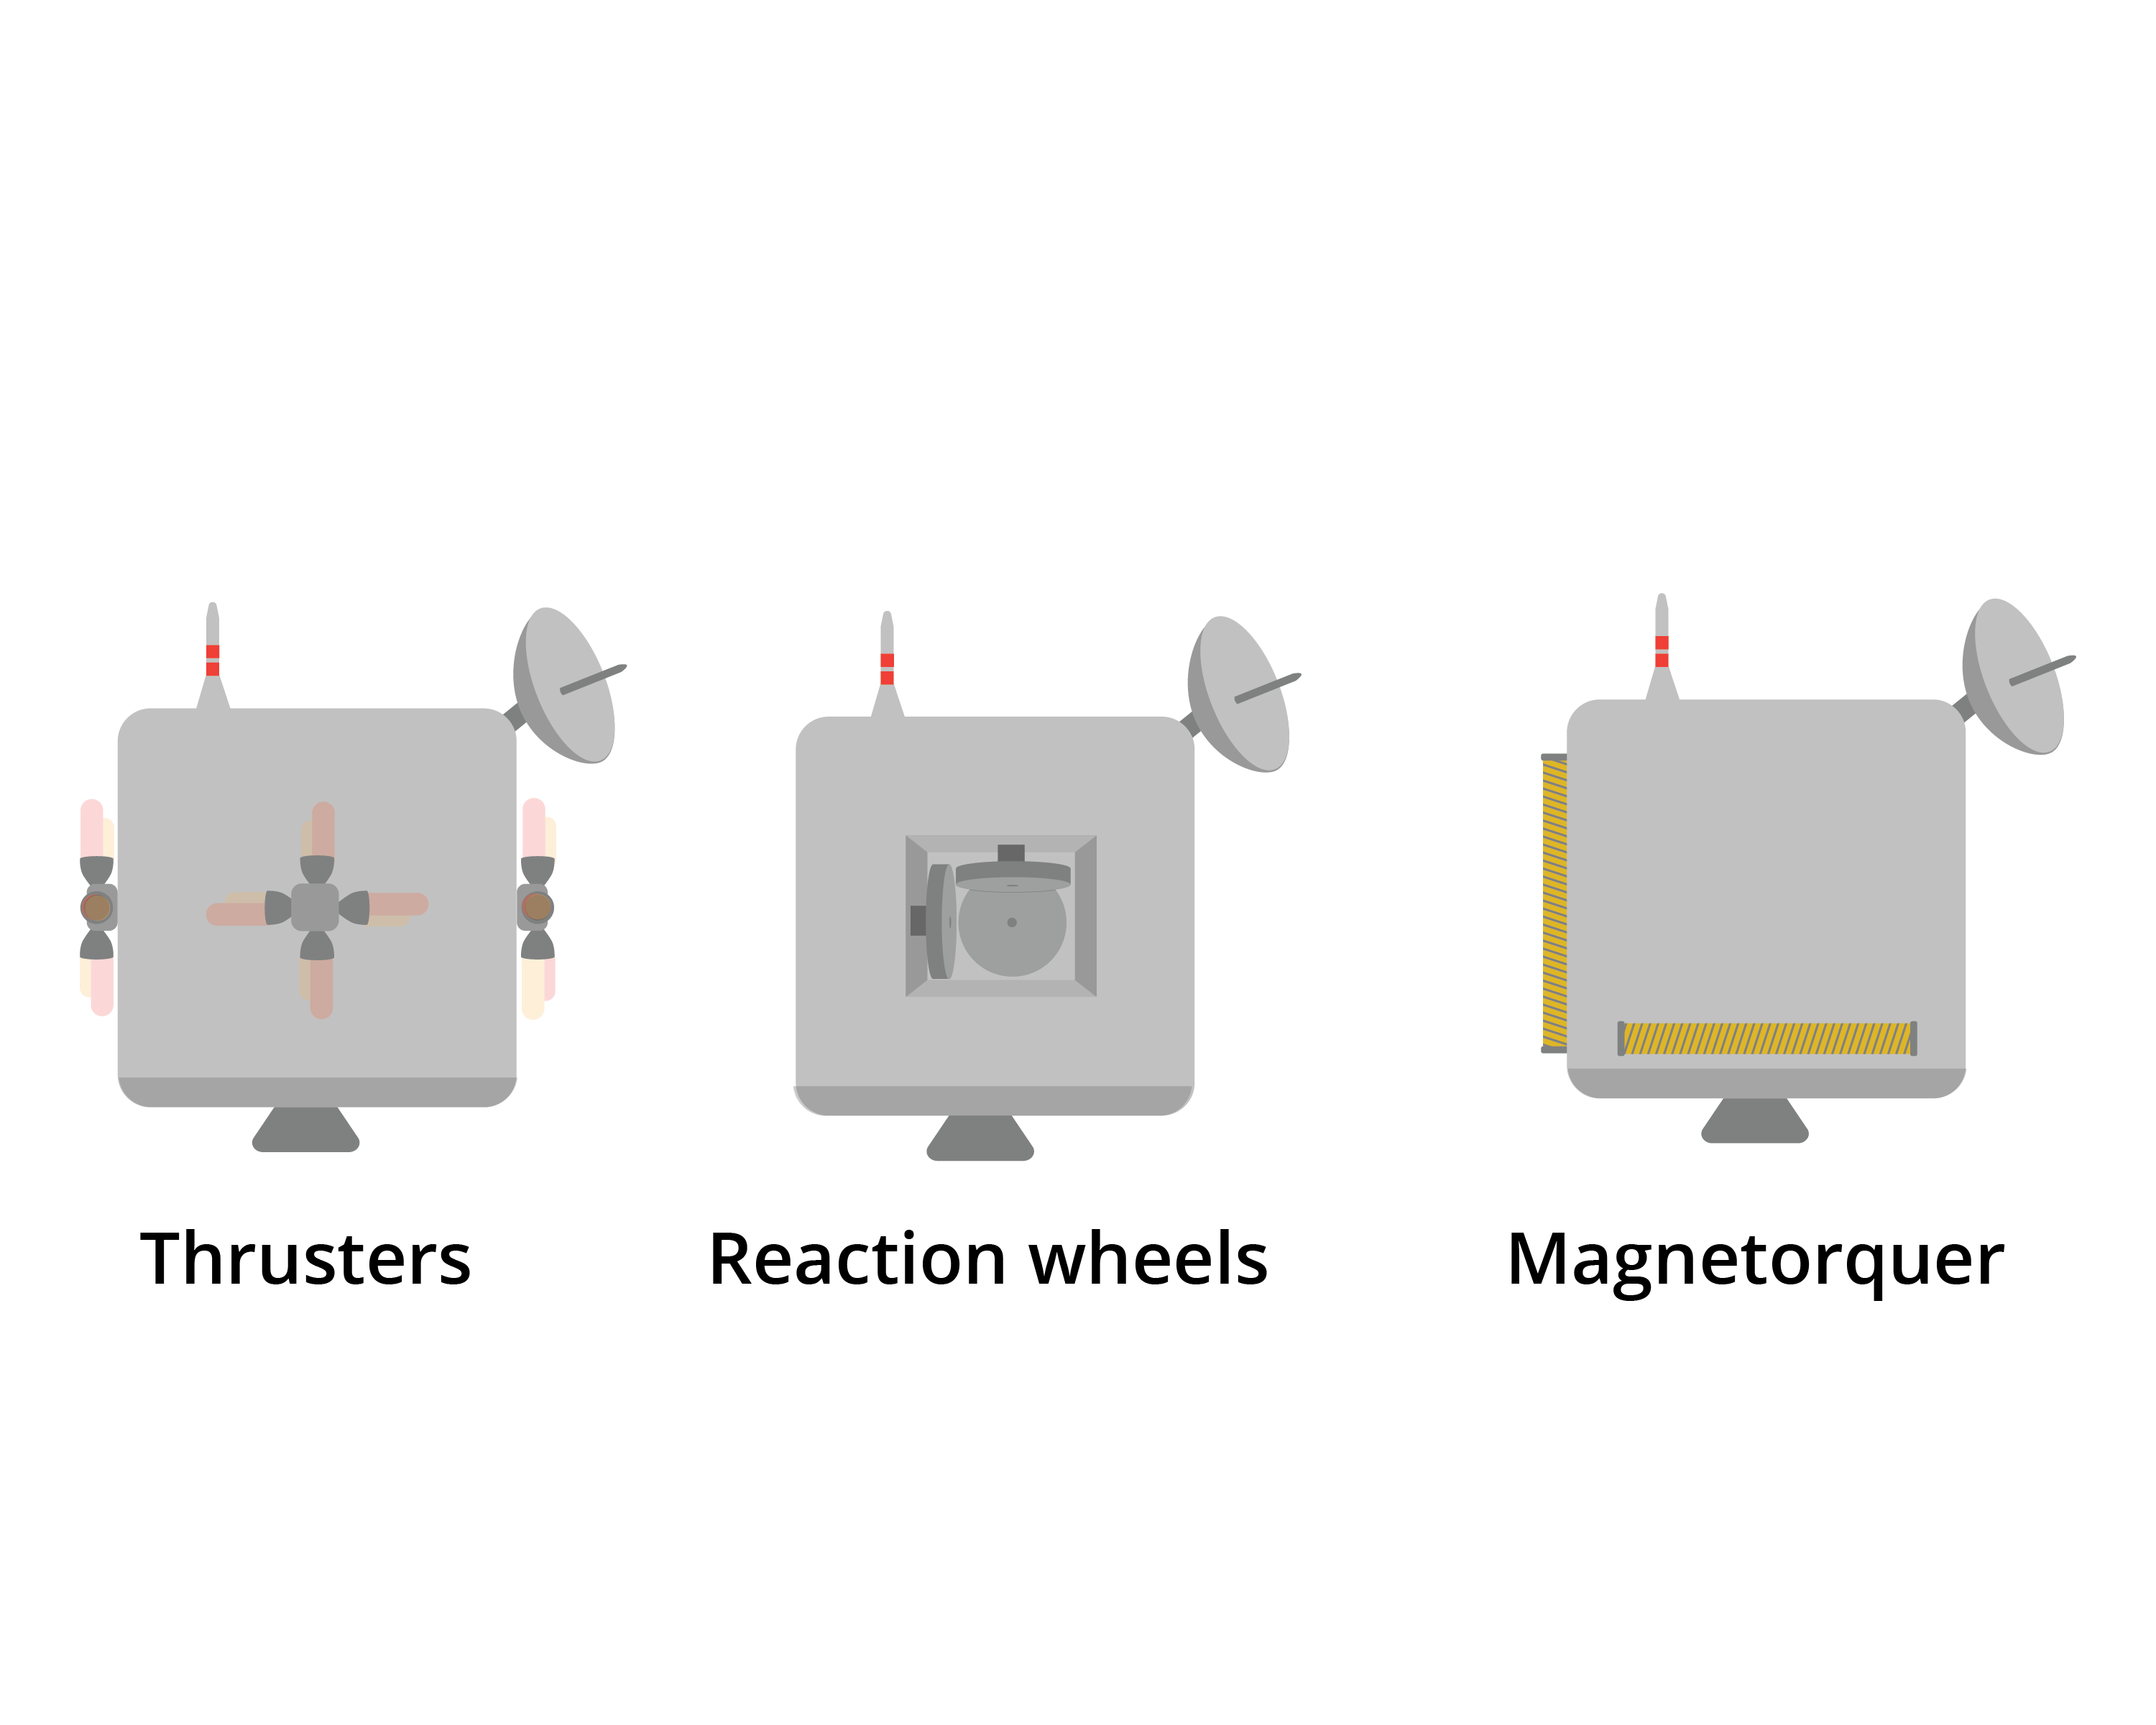
\includegraphics[width=0.75\textwidth]{controlSpace.png}





